%!TEX root = /Users/ego/Boulot/TKZ/tkz-fct/doc-fr/TKZdoc-fct-main.tex    
\section{Macros pour tracer des tangentes }

Si une seule fonction est utilisée, elle est stockée avec comme nom
\tkzcname{tkzFcta}, si une deuxième fonction est utilisée, elle sera stockée avec comme nom \tkzcname{tkzFctb}, et ainsi de suite\ldots Si plusieurs fonctions sont présentent dans un même environnement alors l'option \tkzname{with} permet de choisir celle qui sera mise à contribution.

\tkzHandBomb Il faut bien évidemment, avoir initialisé l'environnement à l'aide \tkzcname{tkzInit}, avant d'appeler \tkzcname{tkzFct} et \tkzcname{tkzDrawTangentLine}. Pour la longueur des vecteurs représentants les demi-tangentes, il faut attribuer une valeur aux coefficients \tkzname{kl} et \tkzname{kr}. $kl=0$ ou $kr=0$ annule le dessin de la demi-tangente correspondante (l=left) et (r=right). Si \tkzname{xstep=1} et \tkzname{ystep=1} alors si la pente est égale à 1, la demi-tangente a pour mesure $\sqrt{2}$.
Dans les autres cas si AT est la longueur de la demi-tangente et si $p$ est la pente alors $\vec{AT}$ a pour coordonnées (\tkzname{kl},\tkzname{kl*p}.) 


\subsection{Représentation d'une tangente \tkzcname{tkzDrawTangentLine}}
\hypertarget{tdtl}{} 
\begin{NewMacroBox}{tkzDrawTangentLine}{\oarg{local options}\parg{a}} 
\emph{On l'emploie soit juste après l'utilisation de \tkzcname{tkzFct}, sinon il faut donner la référence de la fonction à l'aide de l'option \tkzname{with}.}

\medskip
\begin{tabular}{lll}
 \toprule
 options             & exemple & explication    \\ 
 \midrule
 \TAline{a}{\tkzcname{tkzDrawTangentLine(0)}}{tangente au point d'abscisse $0$} 
 \bottomrule
\end{tabular}

Les options sont celles de \TIKZ comme \tkzname{color} ou \tkzname{style} plus les options suivantes

\begin{tabular}{lll}
\toprule
options             & défaut & définition                         \\ 
\midrule
\TOline{draw}{false}{booléen si true alors le point de contact est tracé} 
\TOline{with}{a}{permet de choisir une fonction} 
\TOline{kr}{1}{coefficient pour la longueur de la demi-tangente à droite}
\TOline{kl} {1}{coefficient pour la longueur de la demi-tangente à gauche}
\end{tabular}
\end{NewMacroBox}
%<--------------------------------------------------------------------------->
\subsection{Tangente avec \tkzname{xstep} et \tkzname{ystep} différents de 1}

\begin{tikzpicture}[xscale=1.5]
  \tikzset{tan style/.style={-}}
 \tkzInit[xmin=0,xmax=800,xstep=100,ymin=0,ymax=1800,ystep=400]
 \tkzGrid[color=brown,sub,subxstep=50,subystep=200](0,0)(800,1800)
  \tkzAxeXY
  \tkzFct[color=red,samples=100,domain = 0:800]%
    {(1./90000)*\x*\x*\x-(1./100)*\x*\x+(113./36)*\x}
  \tkzDrawTangentLine[draw,color=blue,kr=300,kl=450,coord](450)
  \tkzText[draw,color = black,fill = brown!50,opacity  = 0.8](300,1200)%
 {$f(x)=\dfrac{1}{90000}x^3 -\dfrac{1}{{100}}x^2 +\dfrac{113}{36}x$}
 \end{tikzpicture}

Il faut remarquer qu'il n'est point nécessaire  de faire des calculs. Il suffit d'utiliser les valeurs qui correspondent aux graduations.

On peut changer le style des tangentes avec,  par exemple,

\tkzcname{tikzset\{tan style/.style=\{-\}\}}  par défaut  on a :

\tkzcname{tikzset\{tan style/.style=\{->,>=latex\}\}}    

\begin{tkzexample}[code only]  
\begin{tikzpicture}[xscale=1.5]
 \tikzset{tan style/.style={-}} 
 \tkzInit[xmin=0,xmax=800,xstep=100,
          ymin=0,ymax=1800,ystep=400]
 \tkzGrid[color=brown,sub,subxstep=50,subystep=200](0,0)(800,1800)
 \tkzAxeXY
 \tkzFct[color=red,samples=100,domain = 0:800]%
    {(1./90000)*\x*\x*\x-(1./100)*\x*\x+(113./36)*\x}
 \tkzDrawTangentLine[color=blue,kr=300,kl=450,coord](450)
 \tkzText[draw, color    = black,%
           fill     = brown!50, opacity  = 0.8](300,1200)%
 {$f(x)=\dfrac{1}{90000}x^3 -\dfrac{1}{{100}}x^2 +\dfrac{113}{36}x$}
 \end{tikzpicture}
 \end{tkzexample}
%<--------------------------------------------------------------------------->     
\subsection{Les options \tkzname{kl}, \tkzname{kr} et l'option \tkzname{draw}}
Si l'un des deux nombres \tkzname{kl} ou \tkzname{kr} est nul alors seulement une demi-tangente est tracée sinon ces nombres représentent un pourcentage de la longueur initiale de la tangente. L'option \tkzname{draw} permet de tracer le point de contact.

\begin{tkzexample}[]
  \begin{tikzpicture}[scale=1.5]
   \tkzInit[xmin=-3,xmax=4,ymin=-4,ymax=2]
   \tkzGrid   \tkzDrawXY \tkzClip
   \tkzFct[domain = -2.15:3.2]{(-x*x)+2*x}
   \tkzDefPointByFct[draw](2)
   \tkzDrawTangentLine[kl=0,draw](-1) 
   \tkzDrawTangentLine[draw](1) 
   \tkzDrawTangentLine[kr=0,draw](3)  
   \tkzRep
 \end{tikzpicture} 
\end{tkzexample}

%<–––––––––––––––––––––––––––––––––––––––––––––––––––––––––––––––––––––––––––>
\subsection{Tangente et l'option \tkzname{with}}
Soit on place la macro  \tkzcname{tkzDrawTangentLine}    après la ligne
 qui définit la première fonction $(a)$, soit  on trace une autre fonction avant, et dans ce cas, il est nécessaire de préciser quelle fonction sera utilisée. pour se faire, on utilise l'option \tkzname{with}.

\begin{tkzexample}[]  
\begin{tikzpicture}[scale=4]
 \tkzInit[xmax=3,ymax=2]
 \tkzAxeXY 
 \tkzGrid(0,0)(3,2)
 \tkzFct[color   = red, domain = 1/3:3]{0.125*(3*x-1)+0.375*(3*x-1)/(x*x)}
 \tkzFct[color   = blue, domain = 1/3:3]{0.125*(3*x-1)}
 \tkzDrawTangentLine[with=a,
                     color=blue](1)
 \tkzText[draw,
          color= red,
          fill=brown!50](1,1.5)%
          {$f(x)=\frac{1}{8}(3x-1)+\frac{3}{8}\left(\frac{3x-1}{x^2}\right)$}
 \tkzText[draw,
          color= green!50!black,
          fill=brown!50](2,0.3)%
          {$g(x)=\frac{1}{8}(3x-1)$}
\end{tikzpicture}
\end{tkzexample}
%<–––––––––––––––––––––––––––––––––––––––––––––––––––––––––––––––––––––––––––>
\subsection{Quelques tangentes }

\begin{tkzexample}[]
\begin{tikzpicture}[scale=2]
  \tkzInit[xmin=-5,xmax=2,ymin=-1, ymax=3]
  \tkzDrawX
  \tkzDrawY
  \tkzText[draw,color = red,fill = orange!20]( 1.5,1.5){$y = xe^x$}
  \tkzFct[color = red, domain = -5:1]{x*exp(x)}%
  \tkzDrawTangentLine[color=blue,kr=2,kl=2](-2)
  \tkzDrawTangentLine[color=green,kr=2,kl=2](-1)
  \tkzDrawTangentLine[color=blue](0)
  \tkzDrawTangentLine[color=blue,kr=0](1)
\end{tikzpicture}
\end{tkzexample}
%<–––––––––––––––––––––––––––––––––––––––––––––––––––––––––––––––––––––––––––>
\subsection{Demi-tangentes }
Il faut remarquer que les tangentes sont en réalité deux demi-tangentes ce qui permet d'obtenir simplement le résultat ci-dessous.

Poosible sont les écritures \tkzname{(((x+1)*x)*x)**0.5},   \tkzname{(x**3+x**2)**0.5} et \tkzname{(x*x*x+x*x)**(0.5)}.

Dans cet exemple, les deux demi-tangentes sont obtenues automatiquement :

\begin{tkzexample}[]
 \begin{tikzpicture}[scale=2.75]
     \tkzInit[xmin=-2,xmax=3,ymax=3]
     \tkzGrid[color=orange](-2,0)(3,3)
     \tkzAxeX
     \tkzAxeY
     \tkzFct[color = red ,domain = -1:2]{(((x+1)*x)*x)**0.5}        
     \tkzDrawTangentLine(0)
     \tkzText[draw,color = red,fill = orange!20](2,1){$f(x)=\sqrt{x^3+x^2}$}
 \end{tikzpicture}
\end{tkzexample}
%<–––––––––––––––––––––––––––––––––––––––––––––––––––––––––––––––––––––––––––>
\subsection{Demi-tangentes Courbe de Lorentz }

Ici, on ne veut que les demi-tangentes comprises entre 0 et 1, pour cela il suffit dans un cas de donner la valeur 0 à \tkzname{kr} et dans l'autre à \tkzname{kl}.

\begin{center}
\begin{tkzexample}[vbox]
\begin{tikzpicture}[scale=1.25]
  \tkzInit[xmax=1,ymax=1,xstep=0.1,ystep=0.1]
  \tkzGrid(0,0)(1,1)
  \tkzAxeXY
  \tkzFct[color = red,thick, domain =0:1]{(exp(\x)-1)/(exp(1)-1)}
  \tkzSetUpPoint[size=12]
  \tkzDrawTangentLine[draw, kl = 0,  kr = 0.4](0)
  \tkzDrawTangentLine[draw, kl = 0.4,kr = 0  ](1)   
  \tkzText[draw,color = red,fill = orange!20](0.5,0.6)%
          {$f(x)=\dfrac{\text{e}^x-1}{\text{e}-1}$}
\end{tikzpicture}
\end{tkzexample}
\end{center}
%<--------------------------------------------------------------------------->
\subsection{Série de tangentes}


\begin{tkzexample}[vbox]  
\begin{tikzpicture}[scale=2]
  \tikzstyle{tan style}=[-]
  \tkzInit[xmin=-5,xmax=2,ymin=-1,ymax=3]
  \tkzDrawXY
  \tkzText[draw,color = red, fill = orange!20](1.5,1.5){$y = xe^x$}
  \tkzFct[line width = 0.01 pt,color = red, domain = -5:1]{x*exp(x)}
  \foreach \x in {-4,-3.8,...,0}{%
    \tkzDrawTangentLine[color=blue,line width=.4pt,kr=1,kl=0.5](\x)}
  \foreach \x in {0.6,0.8,1}{% 
     \tkzDrawTangentLine[color=blue,line width=.4pt, kr=0,kl=0.5](\x)} 
\end{tikzpicture}
\end{tkzexample}
%<--------------------------------------------------------------------------->
\subsection{Série de tangentes sans courbe}

Pour cela, il faut définir la dernière expression avec la syntaxe de \tkzname{fp.sty}.

Définition de \tkzcname{tkzFctLast}
\begin{tkzltxexample}[]
	 \global\edef\tkzFctLast{x*exp(x)} 
\end{tkzltxexample}
	    
\subsubsection{Utilisation de \tkzcname{tkzFctLast}} 
\begin{tkzexample}[vbox]
\begin{tikzpicture}[scale=2]
  \tikzstyle{tan style}=[-]
  \tkzInit[xmin=-5,xmax=2,ymin=-1,ymax=3]
  \tkzDrawXY
  \tkzText[draw,color = red, fill = orange!20](1.5,1.5){$y = xe^x$}
  \global\edef\tkzFctLast{x*exp(x)}% c'est la ligne importante 
  \foreach \v in {-4,-3.8,...,0}{%
    \tkzDrawTangentLine[color=blue,line width=.4pt,kl=1](\v)}
  \foreach \v in {0.6,0.8,1}{% 
    \tkzDrawTangentLine[color=blue,line width=.4pt,kr=0,kl=.75](\v)} 
\end{tikzpicture} 
\end{tkzexample}


\newpage
\subsection{Calcul de l'antécédent}
  
Un problème surgit si on emploie une expression contenant des parenthèses dans l'argument, ainsi \tkzname{(\{1/exp(1)\})} est correct  mais \tkzname{(1/exp(1))} donne une erreur. Il est aussi possible d'évaluer l'antécédent postérieurement comme cela~:
\subsubsection{Valeur numérique de l'antécédent}  
\begin{tkzltxexample}[]  \FPeval\vx{1/exp(1)}
\end{tkzltxexample} 

\subsubsection{utilisation de la valeur numérique} 
\begin{center}
\begin{tkzexample}[]  
\begin{tikzpicture}[scale=1]
  \tkzInit[xmax=1,xstep=0.1,ymin=0.0,ymax=1,ystep=0.1]
  \tkzGrid      \tkzAxeXY
  \tkzFct[domain = 0.00001:1]{(\x**\x)}
  \tkzDrawTangentLine[draw,color = red, kr = 0.2,kl = 0.2]({1/exp(1)}) 
\end{tikzpicture}
\end{tkzexample}
\end{center}



\endinput

